% ============================================================
% Week 3 -- Least squares estimation, estimable linear functions
% ============================================================
\chapter{Linear Models and Estimability}\label{ch:week03}

This chapter covers Week~3 (Lectures 8--10): the one-way classification model, the general
linear model $(Y,X\beta,\sigma^2I_n)$, and the characterisation of estimable linear parametric
functions. From here on, the source for each lecture is the instructor's handwritten notes.
Every step the notes leave as an exercise is proved in full.

% ============================================================
% Lecture 8 -- Fundamentals of Linear Models and the estimation problem
% ============================================================
\section{Fundamentals of Linear Models and the Estimation Problem}\label{sec:L08}

\lectureheader{8}{9RbRhz776-k}{Week-3 handwritten notes \texttt{Feb9.pdf}, first part (``Model 1'', within/between variation, design matrix, identifiability)}

\begin{guiding*}
By the end of this lecture you should be able to:
\begin{itemize}
  \item write down the one-way classification model $Y_{ij}=\mu+\mu_i+\eps_{ij}$ and state the three estimation questions for it;
  \item define $\SSW$, $\SSB$ and $\TSS$, prove $\TSS=\SSW+\SSB$, and state and prove their distributions and independence;
  \item write the model as $Y=X\beta+\eps$, find $\rank(X)$, and explain why its parameters are \emph{not identifiable};
  \item show that contrasts such as $\mu_1-\mu_2$ are identifiable, and that a constraint like $\sum\mu_i=0$ makes all parameters identifiable.
\end{itemize}
\end{guiding*}

\subsection{Motivation}
Week~2 fitted lines to data. From now on we develop the \emph{theory}: when can parameters be
estimated, what is the best estimate, and how are its errors distributed? The instructor begins
with the model that underlies the analysis of variance.

\subsection{The one-way classification model}
\begin{definition}[Model 1: one-way classification]\label{def:L08-oneway}
There are $k$ populations (groups). From population $i$ we observe $n_i$ values $Y_{i1},\dots,Y_{in_i}$:
\[
Y_{ij}=\mu+\mu_i+\eps_{ij},\qquad 1\le i\le k,\quad 1\le j\le n_i,
\]
where $\mu,\mu_1,\dots,\mu_k\in\RR$ are unknown and the errors $\eps_{ij}\sim\N(0,\sigma^2)$ are
independent. The total sample size is $n=n_1+n_2+\dots+n_k$. Here $\mu$ is a general
level and $\mu_i$ the \vocab{effect} of group $i$. The mean of population $i$ is $\mu+\mu_i$.
\end{definition}
The data can be pictured as $k$ columns:
\begin{center}
\begin{tabular}{cccc}\hline
Population 1 & Population 2 & $\cdots$ & Population $k$\\\hline
$Y_{11}$ & $Y_{21}$ & & $Y_{k1}$\\
$\vdots$ & $\vdots$ & & $\vdots$\\
$Y_{1n_1}$ & $Y_{2n_2}$ & & $Y_{kn_k}$\\\hline
\end{tabular}
\end{center}

\begin{question}\label{q:L08-questions}
The lecture poses three questions.
\begin{enumerate}
  \item[(i)] Can we estimate $\mu$? If yes, what is the estimate?
  \item[(ii)] Can we estimate $\mu+\mu_i$? If yes, what is the estimate?
  \item[(iii)] Can we estimate $\mu_i-\mu_j$ for $1\le i\ne j\le k$? If yes, what is the estimate?
\end{enumerate}
\end{question}
The answers are (i) no, (ii) yes, (iii) yes. This lecture shows why (i) fails and gives
unbiased estimates for (iii). \Cref{sec:L10,sec:L13} give the general theory.

\subsection{Within-group and between-group variation}
Write $\bar Y_{i\cdot}=\frac1{n_i}\sum_{j=1}^{n_i}Y_{ij}$ for the mean of group $i$ and
$\bar Y_{\cdot\cdot}=\frac1n\sum_{i=1}^k\sum_{j=1}^{n_i}Y_{ij}$ for the grand mean.

\begin{definition}[Sums of squares]\label{def:L08-SS}
\begin{itemize}
  \item The variance of group $i$ is estimated unbiasedly by the $i$th sample variance
  $S_i^2=\frac{1}{n_i-1}\sum_{j=1}^{n_i}(Y_{ij}-\bar Y_{i\cdot})^2$ (for $n_i\ge 2$).
  \item The \vocab{sum of squares within} groups is $\SSW=\sum_{i=1}^k\sum_{j=1}^{n_i}(Y_{ij}-\bar Y_{i\cdot})^2$.
  \item The \vocab{sum of squares between} groups is $\SSB=\sum_{i=1}^k n_i(\bar Y_{i\cdot}-\bar Y_{\cdot\cdot})^2$.
  \item The \vocab{total sum of squares} is $\TSS=\sum_{i=1}^k\sum_{j=1}^{n_i}(Y_{ij}-\bar Y_{\cdot\cdot})^2$.
\end{itemize}
\end{definition}

\begin{theorem}[Decomposition of the total sum of squares]\label{thm:L08-decomp}
$\TSS=\SSW+\SSB$.
\end{theorem}
\begin{proof}
Write $Y_{ij}-\bar Y_{\cdot\cdot}=(Y_{ij}-\bar Y_{i\cdot})+(\bar Y_{i\cdot}-\bar Y_{\cdot\cdot})$ and square:
\[
\TSS=\sum_{i,j}(Y_{ij}-\bar Y_{i\cdot})^2+\sum_{i,j}(\bar Y_{i\cdot}-\bar Y_{\cdot\cdot})^2
+2\sum_{i=1}^k(\bar Y_{i\cdot}-\bar Y_{\cdot\cdot})\sum_{j=1}^{n_i}(Y_{ij}-\bar Y_{i\cdot}).
\]
The inner sum in the cross term is $\sum_j Y_{ij}-n_i\bar Y_{i\cdot}=0$ for every $i$, so the
cross term vanishes. The first sum is $\SSW$. In the second the summand does not depend on
$j$, so it equals $\sum_i n_i(\bar Y_{i\cdot}-\bar Y_{\cdot\cdot})^2=\SSB$.
\end{proof}

The notes then list distributional facts, the first two posed as exercises. To prove them we
need two tools about normal vectors.

\begin{lemma}[Quadratic forms in projections]\label{lem:L08-chisq}
Let $Z\sim\N(0,I_m)$ (i.e.\ $Z_1,\dots,Z_m$ i.i.d.\ $\N(0,1)$) and let $A$ be an $m\times m$
symmetric matrix with $A^2=A$ and $\rank(A)=r$. Then $Z\T AZ\sim\chi^2_r$.
\end{lemma}
\begin{proof}
By the spectral theorem, $A=Q\Lambda Q\T$ with $Q$ orthogonal and $\Lambda$ diagonal. From
$A^2=A$ we get $\Lambda^2=\Lambda$, so every eigenvalue is $0$ or $1$. The number of $1$'s is
$\rank(\Lambda)=\rank(A)=r$. Order them first. Put $W=Q\T Z$. $W$ is a linear function of a
normal vector, so it is normal, with mean $0$ and covariance $Q\T I Q=I$. Hence
$W_1,\dots,W_m$ are i.i.d.\ $\N(0,1)$, and
$Z\T AZ=W\T\Lambda W=W_1^2+\dots+W_r^2\sim\chi^2_r$.
\end{proof}

\begin{lemma}[Uncorrelated jointly normal vectors are independent]\label{lem:L08-indep}
If $(U,V)$ is jointly normal and $\Cov(U,V)=0$ (every component of $U$ is uncorrelated with
every component of $V$), then $U$ and $V$ are independent. Hence so are $g(U)$ and $h(V)$ for any
functions $g,h$.
\end{lemma}
\begin{proof}
Let $m_U,m_V$ be the means and $\Sigma_U,\Sigma_V$ the covariance matrices. The joint covariance
matrix is block diagonal, $\mathrm{diag}(\Sigma_U,\Sigma_V)$. The moment generating function of a
normal vector $W$ with mean $m$ and covariance $\Sigma$ is $\EE e^{t\T W}=\exp(t\T m+\tfrac12 t\T\Sigma t)$.
For $t=(s,u)$ the block structure gives
\[
\EE e^{s\T U+u\T V}=\exp\bigl(s\T m_U+\tfrac12 s\T\Sigma_Us\bigr)\exp\bigl(u\T m_V+\tfrac12 u\T\Sigma_Vu\bigr)
=\EE e^{s\T U}\,\EE e^{u\T V}.
\]
A joint moment generating function that factorises determines a product distribution, so $U\indep V$.
\end{proof}

\begin{theorem}[Distribution of the sums of squares]\label{thm:L08-dist}
In Model~1:
\begin{enumerate}
  \item $\SSW/\sigma^2\sim\chi^2_{n-k}$: $\SSW$ has $n-k$ \vocab{degrees of freedom};
  \item $\SSW$ is independent of $\SSB$;
  \item if $\mu_1=\mu_2=\dots=\mu_k$, then $\SSB/\sigma^2\sim\chi^2_{k-1}$ ($k-1$ degrees of freedom) and $\TSS/\sigma^2\sim\chi^2_{n-1}$ ($n-1$ degrees of freedom).
\end{enumerate}
\end{theorem}
\begin{proof}
(1) Fix $i$ and let $\eps_i=(\eps_{i1},\dots,\eps_{in_i})\T$. Since $Y_{ij}-\bar Y_{i\cdot}=\eps_{ij}-\bar\eps_{i\cdot}$,
\[
\sum_{j}(Y_{ij}-\bar Y_{i\cdot})^2=\eps_i\T\Bigl(I_{n_i}-\tfrac1{n_i}\one\one\T\Bigr)\eps_i .
\]
The matrix $C_i=I-\frac1{n_i}\one\one\T$ is symmetric and idempotent: $C_i^2=I-\frac2{n_i}\one\one\T+\frac1{n_i^2}\one(\one\T\one)\one\T=C_i$.
Its rank equals its trace, $n_i-1$. The trace equals the rank for idempotent matrices, because
the eigenvalues are $0$ or $1$. Applying \cref{lem:L08-chisq} to $Z=\eps_i/\sigma$ gives
$\sum_j(Y_{ij}-\bar Y_{i\cdot})^2/\sigma^2\sim\chi^2_{n_i-1}$. The $k$ groups are independent. A sum
of independent $\chi^2$ variables is $\chi^2$ with the degrees of freedom added: multiply the
moment generating functions $(1-2t)^{-(n_i-1)/2}$. So $\SSW/\sigma^2\sim\chi^2_{\sum(n_i-1)}=\chi^2_{n-k}$.

(2) $\SSW$ is a function of the vector $U=(\eps_{ij}-\bar\eps_{i\cdot})_{i,j}$. $\SSB$ is a function of
$V=(\bar Y_{1\cdot},\dots,\bar Y_{k\cdot})$, because $\bar Y_{\cdot\cdot}=\frac1n\sum n_i\bar Y_{i\cdot}$. Both are linear
functions of the normal vector $\eps$, so $(U,V)$ is jointly normal. For $i'\ne i$,
$\Cov(\bar Y_{i'\cdot},\eps_{ij}-\bar\eps_{i\cdot})=0$ because different groups are independent. For $i'=i$,
\[
\Cov(\bar\eps_{i\cdot},\eps_{ij}-\bar\eps_{i\cdot})=\Cov(\bar\eps_{i\cdot},\eps_{ij})-\Var(\bar\eps_{i\cdot})=\frac{\sigma^2}{n_i}-\frac{\sigma^2}{n_i}=0 .
\]
By \cref{lem:L08-indep}, $U\indep V$, hence $\SSW\indep\SSB$.

(3) Suppose all $\mu_i$ equal a common value, so every group has mean $\vartheta=\mu+\mu_1$. Then
$\bar Y_{i\cdot}\sim\N(\vartheta,\sigma^2/n_i)$ independently. Put $Z_i=\sqrt{n_i}(\bar Y_{i\cdot}-\vartheta)/\sigma$, so
$Z=(Z_1,\dots,Z_k)\T\sim\N(0,I_k)$. Let $u=(\sqrt{n_1},\dots,\sqrt{n_k})\T/\sqrt n$, a unit vector. By
\cref{prop:L01-bestconst} (with weights $n_i$, same proof),
$\sum_i n_i(\bar Y_{i\cdot}-\vartheta)^2=\SSB+n(\bar Y_{\cdot\cdot}-\vartheta)^2$. Dividing by $\sigma^2$:
\[
\|Z\|^2=\frac{\SSB}{\sigma^2}+(u\T Z)^2,\qquad\text{since } \sqrt n(\bar Y_{\cdot\cdot}-\vartheta)/\sigma=\sum_i\tfrac{\sqrt{n_i}}{\sqrt n}Z_i=u\T Z .
\]
So $\SSB/\sigma^2=Z\T(I_k-uu\T)Z$. The matrix $I_k-uu\T$ is symmetric and idempotent with trace
$k-1$, and \cref{lem:L08-chisq} gives $\chi^2_{k-1}$. Finally $\TSS=\SSW+\SSB$ is a sum of
independent $\chi^2_{n-k}$ and $\chi^2_{k-1}$ variables (times $\sigma^2$), hence $\TSS/\sigma^2\sim\chi^2_{n-1}$.
\end{proof}

\begin{note}
Degrees of freedom: $n-k$ for $\SSW$, $k-1$ for $\SSB$, $n-1$ for $\TSS$, and $(n-k)+(k-1)=n-1$.
Parts of the handwritten notes are hard to read at this point. The degrees of freedom stated
here are the standard ones, and they are the ones the proof gives.
\end{note}

\begin{example}[Sums of squares by hand]\label{ex:L08-SS}
Three groups: group 1 $=\{5,7\}$, group 2 $=\{8,10,12\}$, group 3 $=\{4,6\}$. So $k=3$, $n=7$.
\begin{itemize}
  \item Group means $\bar Y_{1\cdot}=6$, $\bar Y_{2\cdot}=10$, $\bar Y_{3\cdot}=5$. Grand mean $\bar Y_{\cdot\cdot}=52/7=7.4286$.
  \item $\SSW=[(5-6)^2+(7-6)^2]+[(8-10)^2+0+(12-10)^2]+[(4-5)^2+(6-5)^2]=2+8+2=12$.
  \item $\bar Y_{i\cdot}-\bar Y_{\cdot\cdot}=-10/7,\ 18/7,\ -17/7$, so
  $\SSB=\frac{2\cdot100+3\cdot324+2\cdot289}{49}=\frac{1750}{49}=\frac{250}{7}=35.714$.
  \item $\TSS=\SSW+\SSB=12+250/7=334/7=47.714$. Directly: $\sum Y_{ij}^2-n\bar Y_{\cdot\cdot}^2=434-2704/7=334/7$. \checkmark
  \item Degrees of freedom $n-k=4$ and $k-1=2$. The ratio $\frac{\SSB/2}{\SSW/4}=\frac{125/7}{3}=\frac{125}{21}=5.952$ is the $F$ statistic of Week~8. Under equal means it has the $F_{2,4}$ distribution. Here the p-value is $0.063$.
\end{itemize}
\end{example}

\subsection{The model in matrix form}
Stack the data group by group:
$Y=(Y_{11},\dots,Y_{1n_1},\,Y_{21},\dots,Y_{2n_2},\,\dots,\,Y_{k1},\dots,Y_{kn_k})\T\in\RR^n$,
and similarly $\eps$. The parameter vector is $\beta=(\mu,\mu_1,\dots,\mu_k)\T\in\RR^{k+1}$ and
the \vocab{design matrix} is the $n\times(k+1)$ matrix
\[
X=\begin{pmatrix}
\one_{n_1} & \one_{n_1} & 0 & \cdots & 0\\
\one_{n_2} & 0 & \one_{n_2} & \cdots & 0\\
\vdots & & & \ddots & \\
\one_{n_k} & 0 & 0 & \cdots & \one_{n_k}
\end{pmatrix}.
\]
Then $Y_{ij}=\mu+\mu_i+\eps_{ij}$ for all $i,j$ is the same as $Y=X\beta+\eps$, and $\EE[Y]=X\beta$.

\begin{proposition}\label{prop:L08-rank}
If every $n_i\ge 1$, then $\rank(X)=k$, while $X$ has $k+1$ columns.
\end{proposition}
\begin{proof}
Let $c_0$ be the first column and $c_1,\dots,c_k$ the indicator columns of the groups. Every row
has exactly one $1$ among $c_1,\dots,c_k$, so $c_0=c_1+\dots+c_k$ and $\rank(X)=\rank[c_1,\dots,c_k]$.
The columns $c_1,\dots,c_k$ are non-zero ($n_i\ge1$) and have disjoint supports. If
$\sum a_ic_i=0$, then looking at a row of group $i$ gives $a_i=0$. So they are linearly
independent, and $\rank(X)=k$.
\end{proof}

\subsection{Identifiability}
How many parameters are there? $k+1$ (plus $\sigma^2$). Can we estimate all of them? The notes'
answer: \emph{no!} Fix any $c\in\RR$ and set
\[
\tilde\mu=\mu+c,\qquad \tilde\mu_i=\mu_i-c\quad(1\le i\le k).
\]
Then $\tilde\mu+\tilde\mu_i+\eps_{ij}=\mu+\mu_i+\eps_{ij}=Y_{ij}$. The two parameter vectors give
\emph{the same} distribution of the data: ``the models are the same!'' No procedure based on the
data can tell $\mu$ from $\mu+c$.

\begin{definition}[Identifiability]\label{def:L08-ident}
A parameter, or a function $\psi(\beta)$ of the parameters, is \vocab{identifiable} if different
values of it always produce different distributions of the data. In the linear model with
$\EE[Y]=X\beta$, this means: $X\beta_1=X\beta_2\Rightarrow\psi(\beta_1)=\psi(\beta_2)$.
\end{definition}

\begin{example}[What is identifiable in Model 1]\label{ex:L08-ident}
\begin{itemize}
  \item $\mu$ is not identifiable: $\beta_1=(\mu,\mu_1,\dots)$ and $\beta_2=(\mu+c,\mu_1-c,\dots)$ have $X\beta_1=X\beta_2$.
  \item $\mu+\mu_i$ is identifiable. It is the mean of group $i$, which is an entry of $X\beta$.
  \item $\mu_1-\mu_2$ is identifiable. It equals $(\mu+\mu_1)-(\mu+\mu_2)$, a difference of entries of $X\beta$. Moreover $Y_{11}-Y_{21}$ is an \emph{unbiased} estimate: $\EE[Y_{11}-Y_{21}]=(\mu+\mu_1)-(\mu+\mu_2)=\mu_1-\mu_2$.
\end{itemize}
The notes ask: is $Y_{11}-Y_{21}$ \emph{optimal}? What is an optimal estimate? This is answered in
Week~5--6 (BLUEs, the Gauss--Markov theorem). The next note gives a first comparison.
\end{example}

\begin{note}[Supplementary: a better unbiased estimate of $\mu_1-\mu_2$]
$\bar Y_{1\cdot}-\bar Y_{2\cdot}$ is also unbiased for $\mu_1-\mu_2$, and
$\Var(\bar Y_{1\cdot}-\bar Y_{2\cdot})=\sigma^2(1/n_1+1/n_2)\le 2\sigma^2=\Var(Y_{11}-Y_{21})$.
The inequality is strict as soon as $n_1$ or $n_2$ exceeds $1$. Using all the data in each group
beats using one observation. The Gauss--Markov theorem shows that $\bar Y_{1\cdot}-\bar Y_{2\cdot}$ is
in fact the best linear unbiased estimate.
\end{note}

The second way out is a \emph{constraint}. Suppose we assume $\sum_{i=1}^k\mu_i=0$. Then all
parameters become identifiable (``Yay!'' in the notes).

\begin{proposition}\label{prop:L08-constraint}
Under the constraint $\sum_{i=1}^k\mu_i=0$, the map $\beta\mapsto X\beta$ is one-to-one on
$\{\beta:\sum\mu_i=0\}$. Explicitly, if $m_i=\mu+\mu_i$ are the group means, then
$\mu=\frac1k\sum_i m_i$ and $\mu_i=m_i-\frac1k\sum_{l}m_l$.
\end{proposition}
\begin{proof}
$X\beta$ determines the group means $m_i=\mu+\mu_i$. Summing, $\sum_i m_i=k\mu+\sum\mu_i=k\mu$, so
$\mu=\frac1k\sum m_i$, and then $\mu_i=m_i-\mu$. Thus $\beta$ is a function of $X\beta$, and any two
constrained $\beta$ with the same $X\beta$ are equal.
\end{proof}

\begin{note}
In either approach, only $k$ parameters (or combinations of parameters) are identifiable:
the $k$ group means $\mu+\mu_i$ and everything computable from them. The notes ask
\emph{why $k$?} Because $\rank(X)=k$ (\cref{prop:L08-rank}). $X\beta$ ranges over a
$k$-dimensional space, so the data can pin down at most $k$ independent linear combinations of
$\beta$. \Cref{sec:L10} makes this precise.
\end{note}

\subsection{Computation}
The notebook \nb{week03/L08\_oneway\_sums\_of\_squares.ipynb}:
\begin{itemize}
  \item recomputes \cref{ex:L08-SS} and checks it against \texttt{statsmodels}' \texttt{anova\_lm};
  \item builds $X$ for Model~1 and checks $\rank(X)=k$;
  \item shows non-identifiability numerically ($X\beta_1=X\beta_2$ for $\beta_2=\beta_1+c(1,-1,\dots,-1)$);
  \item simulates Model~1 many times and compares the histograms of $\SSW/\sigma^2$ and $\SSB/\sigma^2$ with the $\chi^2_{n-k}$ and $\chi^2_{k-1}$ densities, and checks that their correlation is near $0$.
\end{itemize}

\subsection{Summary}
\begin{itemize}
  \item Model 1: $Y_{ij}=\mu+\mu_i+\eps_{ij}$, $\eps_{ij}$ i.i.d.\ $\N(0,\sigma^2)$, $n=\sum n_i$.
  \item $\TSS=\SSW+\SSB$, with degrees of freedom $n-1=(n-k)+(k-1)$.
  \item $\SSW/\sigma^2\sim\chi^2_{n-k}$ and $\SSW\indep\SSB$. Under equal means, $\SSB/\sigma^2\sim\chi^2_{k-1}$.
  \item $Y=X\beta+\eps$ with $\beta\in\RR^{k+1}$ and $\rank(X)=k$. The parameters are not identifiable ($\mu\to\mu+c$, $\mu_i\to\mu_i-c$).
  \item Group means $\mu+\mu_i$ and contrasts $\mu_i-\mu_j$ are identifiable. The constraint $\sum\mu_i=0$ makes everything identifiable.
\end{itemize}

\subsection{Exercises}
\begin{problem}\label{prob:L08-1}
Show that $S_i^2$ is an unbiased estimate of $\sigma^2$, and that $\SSW/(n-k)$ is unbiased for $\sigma^2$ (without assuming normality).
\end{problem}
\begin{problem}\label{prob:L08-2}
For the groups $\{1,3\}$ and $\{2,4,6\}$ compute $\SSW$, $\SSB$ and $\TSS$ and check \cref{thm:L08-decomp}.
\end{problem}
\begin{problem}\label{prob:L08-3}
Show that in Model 1 (normality not needed) $\EE[\SSB]=(k-1)\sigma^2+\sum_i n_i(\mu_i-\bar\mu_w)^2$, where $\bar\mu_w=\frac1n\sum_i n_i\mu_i$.
\end{problem}
\begin{problem}\label{prob:L08-4}
Prove that the trace of a symmetric idempotent matrix equals its rank.
\end{problem}
\begin{problem}\label{prob:L08-5}
Under the constraint $\sum_i n_i\mu_i=0$ (instead of $\sum_i\mu_i=0$), express $\mu$ and $\mu_i$ in terms of the group means.
\end{problem}

\subsection{Further reading}
Christensen, \S1.2--1.3 (multivariate normal, distribution of quadratic forms), \S2.1
(identifiability and estimability) and Chapter~4 (one-way ANOVA). Rao, \S3b (quadratic forms
in normal variables) and \S4a.

% ============================================================
% Lecture 9 -- Theory of linear models
% ============================================================
\section{Theory of Linear Models}\label{sec:L09}

\lectureheader{9}{kAKqc2ftwaA}{Week-3 handwritten notes \texttt{Feb9.pdf}, part ``Theory of linear models'' (definition, remark, examples, matrix notation)}

\begin{guiding*}
By the end of this lecture you should be able to:
\begin{itemize}
  \item state the general definition of a linear model and explain why it is called \emph{linear};
  \item write the one-way, nested and two-way classification models in this form;
  \item express any linear model in matrix notation as $(Y,X\beta,\sigma^2I_n)$ and compute $\EE[Y]$ and $\Cov(Y)$.
\end{itemize}
\end{guiding*}

\subsection{Recap}
\Cref{sec:L08} studied one particular model, the one-way classification, and wrote it as
$Y=X\beta+\eps$. We now define the general class of models of this kind.

\subsection{Definition}
\begin{definition}[Linear model]\label{def:L09-linmodel}
Suppose we have $n$ observations $\{y_1,\dots,y_n\}$ that are realisations of random variables
$Y_1,\dots,Y_n$. Let $(\beta_1,\dots,\beta_p)$ be the parameters on which the distribution of the
data depends. A \vocab{linear model} is
\[
Y_i=x_{i1}\beta_1+x_{i2}\beta_2+\dots+x_{ip}\beta_p+\eps_i,\qquad 1\le i\le n,
\]
where $\eps_1,\dots,\eps_n$ are \emph{uncorrelated} random variables with $\EE(\eps_i)=0$ and
$\Var(\eps_i)=\sigma^2$ for $1\le i\le n$, and the $x_{ij}$ are known constants.
\end{definition}
(The instructor writes $m$ for the number of parameters. We use $p$; see the notation table.)

\begin{remark}\label{rem:L09-alt}
The model can equivalently be described by
\[
\EE[Y_i]=\sum_{j=1}^p x_{ij}\beta_j\quad(1\le i\le n),\qquad
Y_1,\dots,Y_n \text{ uncorrelated with } \Var(Y_i)=\sigma^2 .
\]
It is called \emph{linear} because the expected value is linear \emph{in the parameters}
$\beta_1,\dots,\beta_p$. It need not be linear in the explanatory variables.
\end{remark}

\begin{note}
Normality is \emph{not} part of the definition. Only means, variances and uncorrelatedness are
assumed. Everything about least squares and the Gauss--Markov theorem needs only these second-order
assumptions. Normality is added later (Week~6, ``Assumption of normality'') to obtain exact
distributions for tests and confidence intervals, as we already did in \cref{thm:L08-dist}.
\end{note}

\begin{example}[Linear in $\beta$, not in $x$]\label{ex:L09-poly}
The quadratic regression $Y_i=\beta_1+\beta_2t_i+\beta_3t_i^2+\eps_i$ is a linear model, with
$x_{i1}=1$, $x_{i2}=t_i$, $x_{i3}=t_i^2$. So is $Y_i=\beta_1+\beta_2\log t_i+\eps_i$. The model
$Y_i=\beta_1e^{\beta_2t_i}+\eps_i$ is \emph{not} linear, because $\beta_2$ enters non-linearly.
\end{example}

\subsection{Examples: classification models}
\begin{example}[One-way classification]\label{ex:L09-oneway}
$Y_{ij}=\mu+\mu_i+\eps_{ij}$, $1\le i\le k$, $1\le j\le n_i$ (\cref{def:L08-oneway}). The
parameters are $(\mu,\mu_1,\dots,\mu_k)$. For observation $(i,j)$ the coefficient of $\mu$ is $1$,
the coefficient of $\mu_i$ is $1$, and all others are $0$.
\end{example}

\begin{example}[Nested classification]\label{ex:L09-nested}
\[
Y_{ijl}=\mu+\mu_i+\delta_{ij}+\eps_{ijl},\qquad 1\le l\le n_{ij},\ 1\le j\le m_i,\ 1\le i\le k .
\]
There are $k$ groups. Group $i$ contains $m_i$ subgroups, and $n_{ij}$ observations are taken in
subgroup $j$ of group $i$. For example, $k$ schools, $m_i$ classes in school $i$, and $n_{ij}$
pupils in class $j$. $\delta_{ij}$ is the effect of subgroup $j$ \emph{within} group $i$. The
subgroups are nested: class 1 of school 1 has nothing to do with class 1 of school 2. The
parameter vector has $1+k+\sum_i m_i$ entries.
\end{example}

\begin{example}[Two-way classification with interaction]\label{ex:L09-twoway}
\[
Y_{ijl}=\mu+\alpha_i+\beta_j+\gamma_{ij}+\eps_{ijl},\qquad 1\le l\le n_{ij},\ 1\le j\le J,\ 1\le i\le I .
\]
Two factors cross each other: factor $A$ with $I$ levels (effects $\alpha_i$) and factor $B$ with
$J$ levels (effects $\beta_j$). $\gamma_{ij}$ is the \emph{interaction}, the extra effect of the
combination $(i,j)$. The notes label this model ``three way classification''. It is the model
the Week-5 assignment calls the two-way classification. There are $1+I+J+IJ$ parameters.
\end{example}

\subsection{Matrix notation}
\begin{definition}[Matrix form]\label{def:L09-matrix}
Put
\[
Y=(Y_1,\dots,Y_n)\T,\quad \beta=(\beta_1,\dots,\beta_p)\T,\quad X=(x_{ij})_{1\le i\le n,\,1\le j\le p},\quad \eps=(\eps_1,\dots,\eps_n)\T .
\]
Then the linear model reads
\[
\underset{n\times1}{Y}=\underset{n\times p}{X}\;\underset{p\times1}{\beta}+\underset{n\times1}{\eps},
\qquad \EE[\eps]=0,\quad \Cov(\eps)=\sigma^2I_n .
\]
We denote it by $(Y,X\beta,\sigma^2I_n)$. The three entries are the observations, their
expectation $\EE[Y]=X\beta$, and the variance--covariance matrix of the data.
\end{definition}

To work with $\Cov$ we recall its definition and the two rules used constantly from now on.
\begin{definition}[Mean vector and covariance matrix]\label{def:L09-cov}
For a random vector $W\in\RR^n$, $\EE[W]=(\EE W_1,\dots,\EE W_n)\T$ and
$\Cov(W)=\EE\bigl[(W-\EE W)(W-\EE W)\T\bigr]$, the $n\times n$ matrix with entries $\Cov(W_i,W_l)$.
\end{definition}

\begin{proposition}\label{prop:L09-rules}
For a random vector $W\in\RR^n$, a fixed $q\times n$ matrix $A$ and a fixed $b\in\RR^q$:
\[
\EE[AW+b]=A\,\EE[W]+b,\qquad \Cov(AW+b)=A\Cov(W)A\T .
\]
In particular, in the linear model $\EE[Y]=X\beta$ and $\Cov(Y)=\sigma^2I_n$.
For a fixed vector $\ell\in\RR^n$, $\EE[\ell\T Y]=\ell\T X\beta$ and $\Var(\ell\T Y)=\sigma^2\pnorm{\ell}^2$.
\end{proposition}
\begin{proof}
The $r$th entry of $AW+b$ is $\sum_l a_{rl}W_l+b_r$. Its expectation is $\sum_l a_{rl}\EE W_l+b_r$
by linearity of expectation, which is the $r$th entry of $A\EE W+b$. Next,
$AW+b-\EE[AW+b]=A(W-\EE W)$, so
\[
\Cov(AW+b)=\EE\bigl[A(W-\EE W)(W-\EE W)\T A\T\bigr]=A\,\EE\bigl[(W-\EE W)(W-\EE W)\T\bigr]A\T=A\Cov(W)A\T ,
\]
again by linearity (entry by entry). For the linear model take $W=\eps$, $A=I$, $b=X\beta$. Then
$Y=\eps+X\beta$ gives $\EE Y=X\beta$ and $\Cov(Y)=\Cov(\eps)=\sigma^2I$. Finally take $A=\ell\T$ ($q=1$):
$\Var(\ell\T Y)=\ell\T(\sigma^2I)\ell=\sigma^2\pnorm{\ell}^2$.
\end{proof}

\begin{example}[Matrix form of simple linear regression]\label{ex:L09-slr}
$Y_i=\beta_1+\beta_2x_i+\eps_i$, $i=1,\dots,4$, with $x=(1,2,3,4)$:
\[
Y=\begin{pmatrix}Y_1\\Y_2\\Y_3\\Y_4\end{pmatrix},\quad
X=\begin{pmatrix}1&1\\1&2\\1&3\\1&4\end{pmatrix},\quad
\beta=\begin{pmatrix}\beta_1\\\beta_2\end{pmatrix},\quad
\EE[Y]=\begin{pmatrix}\beta_1+\beta_2\\\beta_1+2\beta_2\\\beta_1+3\beta_2\\\beta_1+4\beta_2\end{pmatrix},\quad
\Cov(Y)=\sigma^2I_4 .
\]
Here $n=4$, $p=2$ and $\rank(X)=2$. The two columns are not proportional.
\end{example}

\begin{example}[Matrix form of a small nested model]\label{ex:L09-nested-mat}
Take $k=2$ groups, each with $m_i=2$ subgroups and $n_{ij}=1$ observation. With
$\beta=(\mu,\mu_1,\mu_2,\delta_{11},\delta_{12},\delta_{21},\delta_{22})\T$ and
$Y=(Y_{111},Y_{121},Y_{211},Y_{221})\T$:
\[
X=\begin{pmatrix}
1&1&0&1&0&0&0\\
1&1&0&0&1&0&0\\
1&0&1&0&0&1&0\\
1&0&1&0&0&0&1
\end{pmatrix}.
\]
Here $n=4$, $p=7$ and $\rank(X)=4$: the last four columns form $I_4$. There are many more
parameters than identifiable combinations. \Cref{sec:L11} writes out larger examples.
\end{example}

\begin{figure}[ht]
\centering
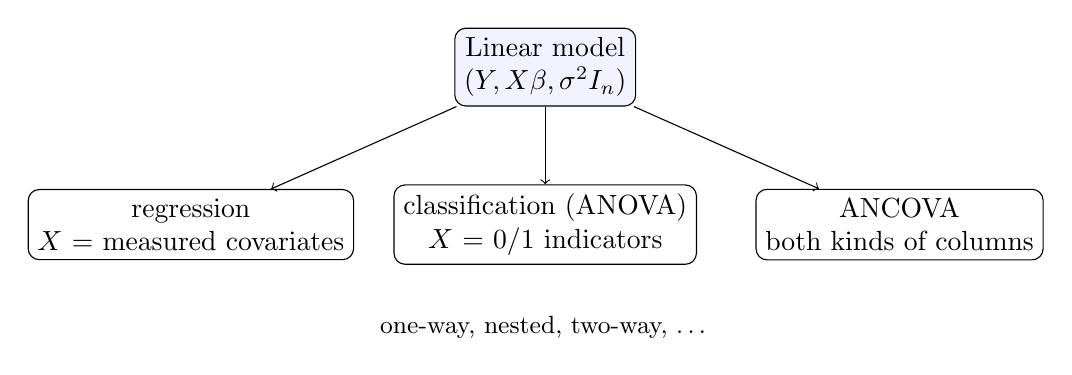
\begin{tikzpicture}[scale=1.0]
\node[draw,rounded corners,fill=blue!5,align=center] (lm) at (0,0) {Linear model\\$(Y,X\beta,\sigma^2I_n)$};
\node[draw,rounded corners,align=center] (reg) at (-4.5,-2) {regression\\$X$ = measured covariates};
\node[draw,rounded corners,align=center] (cls) at (0,-2) {classification (ANOVA)\\$X$ = 0/1 indicators};
\node[draw,rounded corners,align=center] (anc) at (4.5,-2) {ANCOVA\\both kinds of columns};
\draw[->] (lm) -- (reg); \draw[->] (lm) -- (cls); \draw[->] (lm) -- (anc);
\node[font=\small,align=center] at (0,-3.3) {one-way, nested, two-way, \dots};
\end{tikzpicture}
\caption{All models in this course are special cases of $(Y,X\beta,\sigma^2I_n)$. They differ only in the design matrix.}
\label{fig:L09-family}
\end{figure}

\subsection{Computation}
The notebook \nb{week03/L09\_theory\_linear\_models.ipynb} builds the design matrices of
\cref{ex:L09-slr,ex:L09-nested-mat} and of a two-way model with \texttt{numpy}, and also with
\texttt{patsy}/\texttt{statsmodels} formulas. It computes their ranks and checks
$\Cov(AY)=A\Cov(Y)A\T$ by simulation.

\subsection{Summary}
\begin{itemize}
  \item Linear model: $Y_i=\sum_j x_{ij}\beta_j+\eps_i$, with $\eps_i$ uncorrelated, $\EE\eps_i=0$, $\Var\eps_i=\sigma^2$. It is linear in the \emph{parameters}.
  \item Matrix form $(Y,X\beta,\sigma^2I_n)$: $Y=X\beta+\eps$, $\EE Y=X\beta$, $\Cov Y=\sigma^2I_n$.
  \item $\EE[AW+b]=A\EE W+b$ and $\Cov(AW+b)=A\Cov(W)A\T$. In particular $\Var(\ell\T Y)=\sigma^2\pnorm{\ell}^2$.
  \item Classification models (one-way, nested, two-way) are linear models with 0/1 design matrices.
\end{itemize}

\subsection{Exercises}
\begin{problem}\label{prob:L09-1}
Write the design matrix of the two-way model with interaction for $I=J=2$ and $n_{ij}=1$. What is its rank?
\end{problem}
\begin{problem}\label{prob:L09-2}
Which of the following are linear models? (a) $Y_i=\beta_1+\beta_2\sin t_i+\eps_i$; (b) $Y_i=\beta_1t_i^{\beta_2}+\eps_i$; (c) $Y_i=(\beta_1+\beta_2)t_i+\eps_i$.
\end{problem}
\begin{problem}\label{prob:L09-3}
In the linear model, find $\Cov(\bar Y,Y_1-\bar Y)$ where $\bar Y=\frac1n\sum Y_i$.
\end{problem}
\begin{problem}\label{prob:L09-4}
Let $W$ be a random vector with $\Cov(W)=\Sigma$. Show that $\Sigma$ is symmetric and positive semi-definite.
\end{problem}

\subsection{Further reading}
Christensen, \S1.1 (random vectors and matrices) and the introduction to Chapter~2. Rao, \S1b
(matrices) and \S4a.1 (the Gauss--Markoff set-up). Weisberg, \emph{ALR}, Chapter~3.

% ============================================================
% Lecture 10 -- Problem of parameter estimation
% ============================================================
\section{The Problem of Parameter Estimation}\label{sec:L10}

\lectureheader{10}{TnJ_1LZXLBk}{Week-3 handwritten notes \texttt{Feb9.pdf}, part ``The problem of estimation of the parameters'' (linear parametric functions, estimability theorem); Week-5 assignment Q2, Q5, Q6}

\begin{guiding*}
By the end of this lecture you should be able to:
\begin{itemize}
  \item define a \emph{linear parametric function} $\lambda\T\beta$ and say when it is \emph{estimable};
  \item prove that $\lambda\T\beta$ is estimable if and only if $\lambda\in\colsp{X\T}$;
  \item decide estimability in concrete models, including the one-way classification;
  \item relate estimability to the null space of $X$ and to identifiability.
\end{itemize}
\end{guiding*}

\subsection{Recap}
In the linear model $(Y,X\beta,\sigma^2I_n)$ of \cref{sec:L09}, the unknown parameters are
$\beta\in\RR^p$ and $\sigma^2>0$, i.e.\ $(\beta,\sigma^2)\in\RR^p\times\RR_+$. In
\cref{sec:L08} we saw that in the one-way model some linear combinations of $\beta$ (such as
$\mu_1-\mu_2$) have unbiased estimates, while others (such as $\mu$) cannot even be identified.
This lecture characterises the good combinations.

\subsection{Linear parametric functions}
\begin{definition}[Linear parametric function]\label{def:L10-lpf}
For $\lambda=(\lambda_1,\dots,\lambda_p)\T\in\RR^p$, the linear combination
\[
\lambda\T\beta=\lambda_1\beta_1+\lambda_2\beta_2+\dots+\lambda_p\beta_p
\]
of the parameter vector is called a \vocab{linear parametric function}.
\end{definition}
In a linear model we will be interested only in linear parametric functions. The instructor
writes $p\T\beta$ with $p\in\RR^m$; we write $\lambda\T\beta$ because $p$ denotes the number of
parameters in this book.

\begin{definition}[Estimable]\label{def:L10-estimable}
Let $(Y,X\beta,\sigma^2I_n)$ be a linear model and $\lambda\in\RR^p$. The linear parametric function
$\lambda\T\beta$ is \vocab{estimable} if there exists $\ell\in\RR^n$ such that
\[
\EE[\ell\T Y]=\lambda\T\beta\qquad\text{for every }\beta\in\RR^p .
\]
In other words, $\lambda\T\beta$ is estimable if it has a \emph{linear unbiased estimate} $\ell\T Y$.
\end{definition}
Unbiasedness must hold for every value of $\beta$. An estimate that is unbiased only for some
$\beta$'s is useless, because we do not know $\beta$.

\subsection{The estimability theorem}
\begin{theorem}[Characterisation of estimability]\label{thm:L10-estimable}
Let $(Y,X\beta,\sigma^2I_n)$ be a linear model and $\lambda\in\RR^p$. Then
\[
\lambda\T\beta \text{ is estimable}\iff \lambda\in\colsp{X\T},
\]
where $\colsp{X\T}=\{z\in\RR^p:\ z=X\T\ell\text{ for some }\ell\in\RR^n\}$ is the column space of
$X\T$, which is the row space of $X$.
\end{theorem}
\begin{proof}
We follow the chain of equivalences in the notes and justify each step.
\begin{align*}
\lambda\T\beta\text{ estimable}
&\iff \exists\,\ell\in\RR^n:\ \EE[\ell\T Y]=\lambda\T\beta\ \ \forall\beta\in\RR^p &&\text{(definition)}\\
&\iff \exists\,\ell\in\RR^n:\ \ell\T X\beta=\lambda\T\beta\ \ \forall\beta\in\RR^p &&\text{(linearity of expectation)}\\
&\iff \exists\,\ell\in\RR^n:\ X\T\ell=\lambda &&\text{(linear algebra, below)}\\
&\iff \lambda\in\colsp{X\T}. &&\text{(definition of column space)}
\end{align*}
Step 2: $\EE[\ell\T Y]=\ell\T\EE[Y]=\ell\T X\beta$ by \cref{prop:L09-rules}.
Step 3: $\ell\T X\beta=\lambda\T\beta$ for all $\beta$ means $(X\T\ell-\lambda)\T\beta=0$ for all $\beta$.
Taking $\beta=X\T\ell-\lambda$ gives $\pnorm{X\T\ell-\lambda}^2=0$, i.e.\ $X\T\ell=\lambda$. Conversely,
if $X\T\ell=\lambda$ then $\ell\T X\beta=(X\T\ell)\T\beta=\lambda\T\beta$ for all $\beta$.
\end{proof}

\begin{note}
The proof shows more than the statement. The linear unbiased estimates of $\lambda\T\beta$ are
\emph{exactly} the $\ell\T Y$ with $X\T\ell=\lambda$ (this is Week-5 assignment Q2). If some
$\ell_0$ works, then so does $\ell_0+v$ for every $v\in\nullsp{X\T}$. So there are usually many
linear unbiased estimates, and the question ``which one is best?'' (Weeks~5--6) makes sense.
\end{note}

\begin{corollary}\label{cor:L10-fullrank}
Every linear parametric function is estimable $\iff\colsp{X\T}=\RR^p\iff\rank(X)=p$.
In that case the parameters $\beta_1,\dots,\beta_p$ themselves are estimable.
\end{corollary}
\begin{proof}
All $\lambda$ lie in $\colsp{X\T}$ iff $\colsp{X\T}=\RR^p$, i.e.\ iff $\dim\colsp{X\T}=\rank(X)=p$.
Then $\beta_j=e_j\T\beta$ is estimable for each standard basis vector $e_j$.
\end{proof}

\begin{corollary}[Estimable functions form a subspace]\label{cor:L10-subspace}
If $\lambda_1\T\beta$ and $\lambda_2\T\beta$ are estimable, so is $(a\lambda_1+b\lambda_2)\T\beta$ for all
$a,b\in\RR$. Each row $x_i\T\beta=\EE Y_i$ of $X\beta$ is estimable (take $\ell=e_i$). Every estimable
function is a linear combination of these.
\end{corollary}
\begin{proof}
$\colsp{X\T}$ is a subspace spanned by the rows $x_1,\dots,x_n$ of $X$. If
$\lambda_1=X\T\ell_1$ and $\lambda_2=X\T\ell_2$ then $a\lambda_1+b\lambda_2=X\T(a\ell_1+b\ell_2)$.
\end{proof}

\begin{proposition}[Week-5 assignment Q5]\label{prop:L10-nullspace}
$\lambda\T\beta$ is estimable $\iff$ $\lambda$ is orthogonal to the null space $\nullsp{X}=\{v:Xv=0\}$.
\end{proposition}
\begin{proof}
By \cref{thm:L10-estimable} we must show $\colsp{X\T}=\nullsp{X}^\perp$.
($\subseteq$) If $\lambda=X\T\ell$ and $Xv=0$, then $\lambda\T v=\ell\T Xv=0$.
($\supseteq$) Both are subspaces of $\RR^p$. $\dim\colsp{X\T}=\rank(X)=r$, and by rank--nullity
$\dim\nullsp{X}=p-r$, so $\dim\nullsp{X}^\perp=r$. A subspace contained in another of the same
finite dimension equals it.
\end{proof}

\begin{note}[Supplementary: estimable $\Rightarrow$ identifiable]
If $\lambda\T\beta$ is estimable and $X\beta_1=X\beta_2$, then $\beta_1-\beta_2\in\nullsp{X}$, so
$\lambda\T\beta_1=\lambda\T\beta_2$ by \cref{prop:L10-nullspace}. Estimable functions are therefore
identifiable in the sense of \cref{def:L08-ident}. Conversely, a linear function that is
identifiable (constant on each set $\{\beta: X\beta=\text{const}\}$) must vanish on $\nullsp{X}$, so it
is estimable. For linear parametric functions the two notions coincide.
\end{note}

\subsection{Examples}
\begin{example}[One-way model with $k=2$, $n_1=n_2=2$]\label{ex:L10-oneway}
With $\beta=(\mu,\mu_1,\mu_2)\T$ and $Y=(Y_{11},Y_{12},Y_{21},Y_{22})\T$,
\[
X=\begin{pmatrix}1&1&0\\1&1&0\\1&0&1\\1&0&1\end{pmatrix},\qquad
\colsp{X\T}=\mathrm{span}\{(1,1,0)\T,(1,0,1)\T\}.
\]
\begin{itemize}
  \item $\mu_1-\mu_2$: $\lambda=(0,1,-1)\T=(1,1,0)\T-(1,0,1)\T\in\colsp{X\T}$, so it is \emph{estimable}. Two linear unbiased estimates are $\ell=(1,0,-1,0)\T$, i.e.\ $Y_{11}-Y_{21}$, and $\ell=(\tfrac12,\tfrac12,-\tfrac12,-\tfrac12)\T$, i.e.\ $\bar Y_{1\cdot}-\bar Y_{2\cdot}$. Both satisfy $X\T\ell=(0,1,-1)\T$. Their variances are $\sigma^2\pnorm{\ell}^2=2\sigma^2$ and $\sigma^2$ respectively.
  \item $\mu+\mu_1$: $\lambda=(1,1,0)\T$ is a row of $X$, so it is \emph{estimable} (e.g.\ by $Y_{11}$, or better by $\bar Y_{1\cdot}$).
  \item $\mu_1$: $\lambda=(0,1,0)\T$. If $a(1,1,0)+b(1,0,1)=(0,1,0)$ then $a+b=0$, $a=1$, $b=0$, a contradiction. So it is \emph{not estimable}. Equivalently, $\nullsp{X}=\mathrm{span}\{(1,-1,-1)\T\}$ and $\lambda\T(1,-1,-1)\T=-1\ne0$.
  \item $\mu$: $\lambda=(1,0,0)\T$ has $\lambda\T(1,-1,-1)\T=1\ne 0$, so it is \emph{not estimable}.
\end{itemize}
\end{example}

\begin{example}[General one-way model]\label{ex:L10-oneway-general}
In Model~1 with $\beta=(\mu,\mu_1,\dots,\mu_k)\T$, the rows of $X$ are $(1,e_i\T)$. By
\cref{prop:L08-rank}, $\nullsp{X}$ is one-dimensional, spanned by $v=(1,-1,\dots,-1)\T$.
Hence, by \cref{prop:L10-nullspace},
\[
\lambda_0\mu+\sum_{i=1}^k\lambda_i\mu_i\ \text{is estimable}\iff \lambda_0=\sum_{i=1}^k\lambda_i .
\]
Consequences: any \vocab{contrast} $\sum\lambda_i\mu_i$ with $\sum\lambda_i=0$ is estimable (e.g.\
$\mu_1-\mu_2$, $\mu_1+\mu_2-2\mu_3$), and so is $\mu+\mu_i$. The functions $\mu$ and $\mu_i$ alone are not.
This answers \cref{q:L08-questions}.
\end{example}

\begin{figure}[ht]
\centering
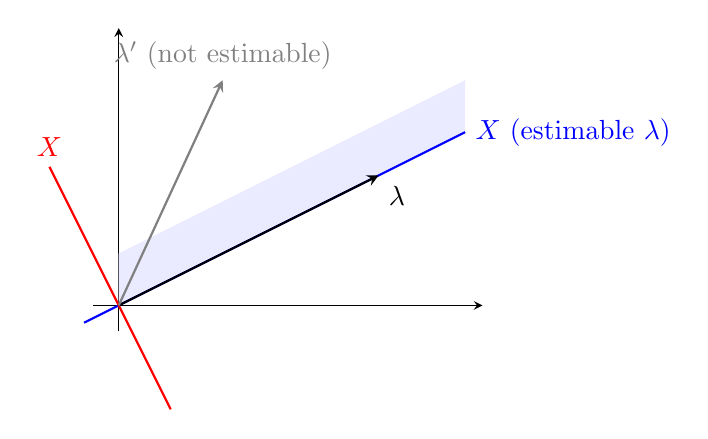
\begin{tikzpicture}[scale=1.1,>=stealth]
\draw[->] (-0.3,0) -- (4.2,0) node[right] {};
\draw[->] (0,-0.3) -- (0,3.2);
\fill[blue!8] (0,0) -- (4,2) -- (4,2.6) -- (0,0.6) -- cycle;
\draw[thick,blue] (-0.4,-0.2) -- (4,2) node[right] {$\colsp{X\T}$ (estimable $\lambda$)};
\draw[thick,red] (0.6,-1.2) -- (-0.8,1.6) node[above] {$\nullsp{X}$};
\draw[->,thick] (0,0) -- (3,1.5) node[below right] {$\lambda$};
\draw[->,thick,gray] (0,0) -- (1.2,2.6) node[above] {$\lambda'$ (not estimable)};
\end{tikzpicture}
\caption{$\lambda\T\beta$ is estimable exactly when $\lambda$ lies in the row space $\colsp{X\T}=\nullsp{X}^\perp$ (schematic, $p=2$, $\rank X=1$).}
\label{fig:L10-geom}
\end{figure}

\subsection{Computation}
To test whether $\lambda\in\colsp{X\T}$ numerically, compare $\rank(X\T)$ with $\rank([X\T\ \lambda])$,
or check whether $\lambda$ is orthogonal to a basis of $\nullsp{X}$ (\texttt{scipy.linalg.null\_space}).
A third test uses the Moore--Penrose inverse: $\lambda\in\colsp{X\T}\iff X\T(X\T)^{+}\lambda=\lambda$.
All three are implemented, and checked on \cref{ex:L10-oneway}, in
\nb{week03/L10\_estimability.ipynb}. The notebook also finds $\ell$ with $X\T\ell=\lambda$ and
verifies unbiasedness by simulation.

\subsection{Summary}
\begin{itemize}
  \item Linear parametric function: $\lambda\T\beta$. Estimable: $\exists\,\ell$ with $\EE[\ell\T Y]=\lambda\T\beta$ for all $\beta$.
  \item \textbf{Theorem:} $\lambda\T\beta$ is estimable $\iff\lambda\in\colsp{X\T}\iff\lambda\perp\nullsp{X}$. The linear unbiased estimates are $\ell\T Y$ with $X\T\ell=\lambda$.
  \item If $\rank X=p$, everything is estimable. Estimable functions form the $r$-dimensional space spanned by the rows of $X$.
  \item One-way model: $\lambda_0\mu+\sum\lambda_i\mu_i$ is estimable iff $\lambda_0=\sum\lambda_i$.
\end{itemize}

\subsection{Exercises}
\begin{problem}\label{prob:L10-1}
In the one-way model with $k=3$, decide which are estimable: $\mu$, $\mu_1-\mu_2$, $\mu+\mu_1$, $\mu_1+\mu_2-2\mu_3$, $2\mu+\mu_1+\mu_2$.
\end{problem}
\begin{problem}\label{prob:L10-2}
(Week-5 assignment Q6.) Let $k,l\ge 2$ be integers and let $X$ have rows $(1,i,ik)$ for $i=1,\dots,k$ followed by rows $(1,i,il)$ for $i=1,\dots,l$, with $\beta=(\beta_1,\beta_2,\beta_3)\T$.
(a) Show that $\beta_1$ and $\beta_2+\beta_3(l+k)/2$ are always estimable.
(b) Find a necessary and sufficient condition on $k,l$ for every linear function of $\beta$ to be estimable.
\end{problem}
\begin{problem}\label{prob:L10-3}
Show that if $\lambda\T\beta$ is estimable, then any two linear unbiased estimates $\ell_1\T Y,\ell_2\T Y$ differ by $v\T Y$ with $v\in\nullsp{X\T}$, and that $\EE[v\T Y]=0$.
\end{problem}
\begin{problem}\label{prob:L10-4}
In simple linear regression $Y_i=\beta_1+\beta_2x_i+\eps_i$, when is $\beta_2$ estimable? Relate your answer to \cref{prob:L05-4}.
\end{problem}
\begin{problem}\label{prob:L10-5}
In the nested model of \cref{ex:L09-nested-mat}, show that $\delta_{11}-\delta_{12}$ is estimable but $\mu_1-\mu_2$ is not.
\end{problem}

\subsection{Further reading}
Christensen, \S2.1 (Identifiability and Estimability), especially the result that $\lambda\T\beta$
is estimable iff $\lambda\T=\rho\T X$ for some $\rho$. Rao, \S4a.1 (estimable parametric functions).


\section*{Solutions to the Exercises of Chapter~\ref{ch:week03}}
\addcontentsline{toc}{section}{Solutions to the exercises}

\paragraph{\Cref{prob:L08-1}.}
Within group $i$, $\sum_j(Y_{ij}-\bar Y_{i\cdot})^2=\sum_j(\eps_{ij}-\bar\eps_{i\cdot})^2=\sum_j\eps_{ij}^2-n_i\bar\eps_{i\cdot}^2$.
Taking expectations, $\EE\sum_j\eps_{ij}^2=n_i\sigma^2$ and $\EE[n_i\bar\eps_{i\cdot}^2]=n_i\Var(\bar\eps_{i\cdot})=\sigma^2$.
So the expectation is $(n_i-1)\sigma^2$, and $\EE S_i^2=\sigma^2$. Summing over groups,
$\EE\,\SSW=\sum_i(n_i-1)\sigma^2=(n-k)\sigma^2$. Only $\EE\eps=0$, $\Var\eps_{ij}=\sigma^2$ and
uncorrelatedness were used.

\paragraph{\Cref{prob:L08-2}.}
Means: $2$ and $4$; grand mean $16/5=3.2$. $\SSW=(1+1)+(4+0+4)=10$.
$\SSB=2(2-3.2)^2+3(4-3.2)^2=2.88+1.92=4.8$.
$\TSS=(1-3.2)^2+(3-3.2)^2+(2-3.2)^2+(4-3.2)^2+(6-3.2)^2=4.84+0.04+1.44+0.64+7.84=14.8=10+4.8$. \checkmark

\paragraph{\Cref{prob:L08-3}.}
Let $m_i=\mu+\mu_i$ and $\bar m=\frac1n\sum n_im_i=\mu+\bar\mu_w$. Write
$\bar Y_{i\cdot}=m_i+\bar\eps_{i\cdot}$ and $\bar Y_{\cdot\cdot}=\bar m+\bar\eps_{\cdot\cdot}$. By the weighted version of
\cref{prop:L01-bestconst}, $\SSB=\sum n_i\bar Y_{i\cdot}^2-n\bar Y_{\cdot\cdot}^2$.
Now $\EE\bar Y_{i\cdot}^2=m_i^2+\sigma^2/n_i$ and $\EE\bar Y_{\cdot\cdot}^2=\bar m^2+\sigma^2/n$. Hence
$\EE\,\SSB=\sum n_im_i^2+k\sigma^2-n\bar m^2-\sigma^2=(k-1)\sigma^2+\sum n_i(m_i-\bar m)^2$, and
$m_i-\bar m=\mu_i-\bar\mu_w$.

\paragraph{\Cref{prob:L08-4}.}
From the proof of \cref{lem:L08-chisq}, $A=Q\Lambda Q\T$ with $\Lambda$ diagonal with $0/1$ entries.
Then $\tr A=\tr(\Lambda Q\T Q)=\tr\Lambda=$ the number of $1$'s $=\rank\Lambda=\rank A$.

\paragraph{\Cref{prob:L08-5}.}
$\sum_i n_im_i=n\mu+\sum n_i\mu_i=n\mu$. So $\mu=\frac1n\sum n_im_i$, which is the weighted average of
the group means, and $\mu_i=m_i-\mu$.

\paragraph{\Cref{prob:L09-1}.}
Order the observations as $(1,1)$, $(1,2)$, $(2,1)$, $(2,2)$ and the parameters as
$\mu$, $\alpha_1$, $\alpha_2$, $\beta_1$, $\beta_2$, $\gamma_{11}$, $\gamma_{12}$, $\gamma_{21}$, $\gamma_{22}$:
\[
X=\begin{pmatrix}
1&1&0&1&0&1&0&0&0\\
1&1&0&0&1&0&1&0&0\\
1&0&1&1&0&0&0&1&0\\
1&0&1&0&1&0&0&0&1
\end{pmatrix},\qquad \rank X=4
\]
(the $\gamma$ columns form $I_4$), while $p=9$.

\paragraph{\Cref{prob:L09-2}.}
(a) Linear, with $x_{i2}=\sin t_i$. (b) Not linear, because $\beta_2$ is in the exponent.
(c) The mean $(\beta_1+\beta_2)t_i$ is linear in $(\beta_1,\beta_2)$, so it is formally a linear model with
$x_{i1}=x_{i2}=t_i$. The design matrix has two equal columns, and only $\beta_1+\beta_2$ is estimable.

\paragraph{\Cref{prob:L09-3}.}
$\Cov(\bar Y,Y_1)=\frac1n\sum_l\Cov(Y_l,Y_1)=\sigma^2/n$ and $\Var(\bar Y)=\sigma^2/n$, so
$\Cov(\bar Y,Y_1-\bar Y)=0$.

\paragraph{\Cref{prob:L09-4}.}
Symmetry: $\Cov(W_i,W_l)=\Cov(W_l,W_i)$. For any $a\in\RR^n$,
$a\T\Sigma a=\Var(a\T W)\ge 0$ by \cref{prop:L09-rules}.

\paragraph{\Cref{prob:L10-1}.}
Use \cref{ex:L10-oneway-general}: $\lambda_0\mu+\sum\lambda_i\mu_i$ is estimable iff $\lambda_0=\sum\lambda_i$.
$\mu$: $1\ne0$, not estimable. $\mu_1-\mu_2$: $0=1-1$, estimable. $\mu+\mu_1$: $1=1$, estimable.
$\mu_1+\mu_2-2\mu_3$: $0=0$, estimable. $2\mu+\mu_1+\mu_2$: $2=2$, estimable. It is $(\mu+\mu_1)+(\mu+\mu_2)$.

\paragraph{\Cref{prob:L10-2}.}
Each row $(1,i,ik)=(1,0,0)+i(0,1,k)$. Since $k\ge2$, the first block contains $i=1,2$, whose rows
span $\{(1,0,0),(0,1,k)\}$. Similarly the second block spans $\{(1,0,0),(0,1,l)\}$. So
$\colsp{X\T}=\mathrm{span}\{(1,0,0),(0,1,k),(0,1,l)\}$.
(a) $(1,0,0)\T$ is in it, so $\beta_1$ is estimable. Also $(0,1,\frac{k+l}2)=\frac12(0,1,k)+\frac12(0,1,l)$ is in it,
so $\beta_2+\beta_3(k+l)/2$ is estimable, whatever $k,l$ are.
(b) $(0,1,k)$ and $(0,1,l)$ are linearly independent iff $k\ne l$. So $\rank X=3$, and every linear
function is estimable (\cref{cor:L10-fullrank}), iff $k\ne l$. If $k=l$, $\rank X=2$ and e.g.\ $\beta_3$ is
not estimable.

\paragraph{\Cref{prob:L10-3}.}
$X\T\ell_1=\lambda=X\T\ell_2$ gives $X\T(\ell_1-\ell_2)=0$, i.e.\ $v=\ell_1-\ell_2\in\nullsp{X\T}$.
Then $\EE[v\T Y]=v\T X\beta=(X\T v)\T\beta=0$.

\paragraph{\Cref{prob:L10-4}.}
$X=[\one,x]$. If the $x_i$ are not all equal, $\rank X=2=p$ and $\beta_2$ is estimable. If all
$x_i=c$, the rows are all $(1,c)$, so $\colsp{X\T}=\mathrm{span}\{(1,c)\}$. Then $(0,1)$ is not in it, and $\beta_2$
is not estimable. This matches \cref{prob:L05-4}, where the least-squares slope was not unique.

\paragraph{\Cref{prob:L10-5}.}
$\lambda=(0,0,0,1,-1,0,0)\T$ equals row 1 $-$ row 2 of $X$, so $\delta_{11}-\delta_{12}$ is estimable (by
$Y_{111}-Y_{121}$). For $\mu_1-\mu_2$, $\lambda=(0,1,-1,0,0,0,0)\T$. The vector
$v=(0,1,0,-1,-1,0,0)\T$ satisfies $Xv=0$: rows 1 and 2 give $1-1=0$, and rows 3 and 4 give $0$. But
$\lambda\T v=1\ne0$, so by \cref{prop:L10-nullspace} $\mu_1-\mu_2$ is not estimable. Only
combinations such as $(\mu_1+\frac12(\delta_{11}+\delta_{12}))-(\mu_2+\frac12(\delta_{21}+\delta_{22}))$ are estimable.
